\documentclass{article}
\usepackage{graphicx}
\usepackage{csvsimple}
\graphicspath{ {./images/} }
\title{\textbf{DTL Assignment 3}}
\date{2022-02-11}
\author{Mohit Apte MIS - 112103012}
\begin{document}
\maketitle
\begin{LARGE}
\begin{center}
USE OF TABLES AND IMAGES IN LATEX
\end{center}
\end{LARGE}
\pagenumbering{roman}
\newpage
\begin{center}
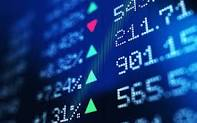
\includegraphics[width=\textwidth]{stock}
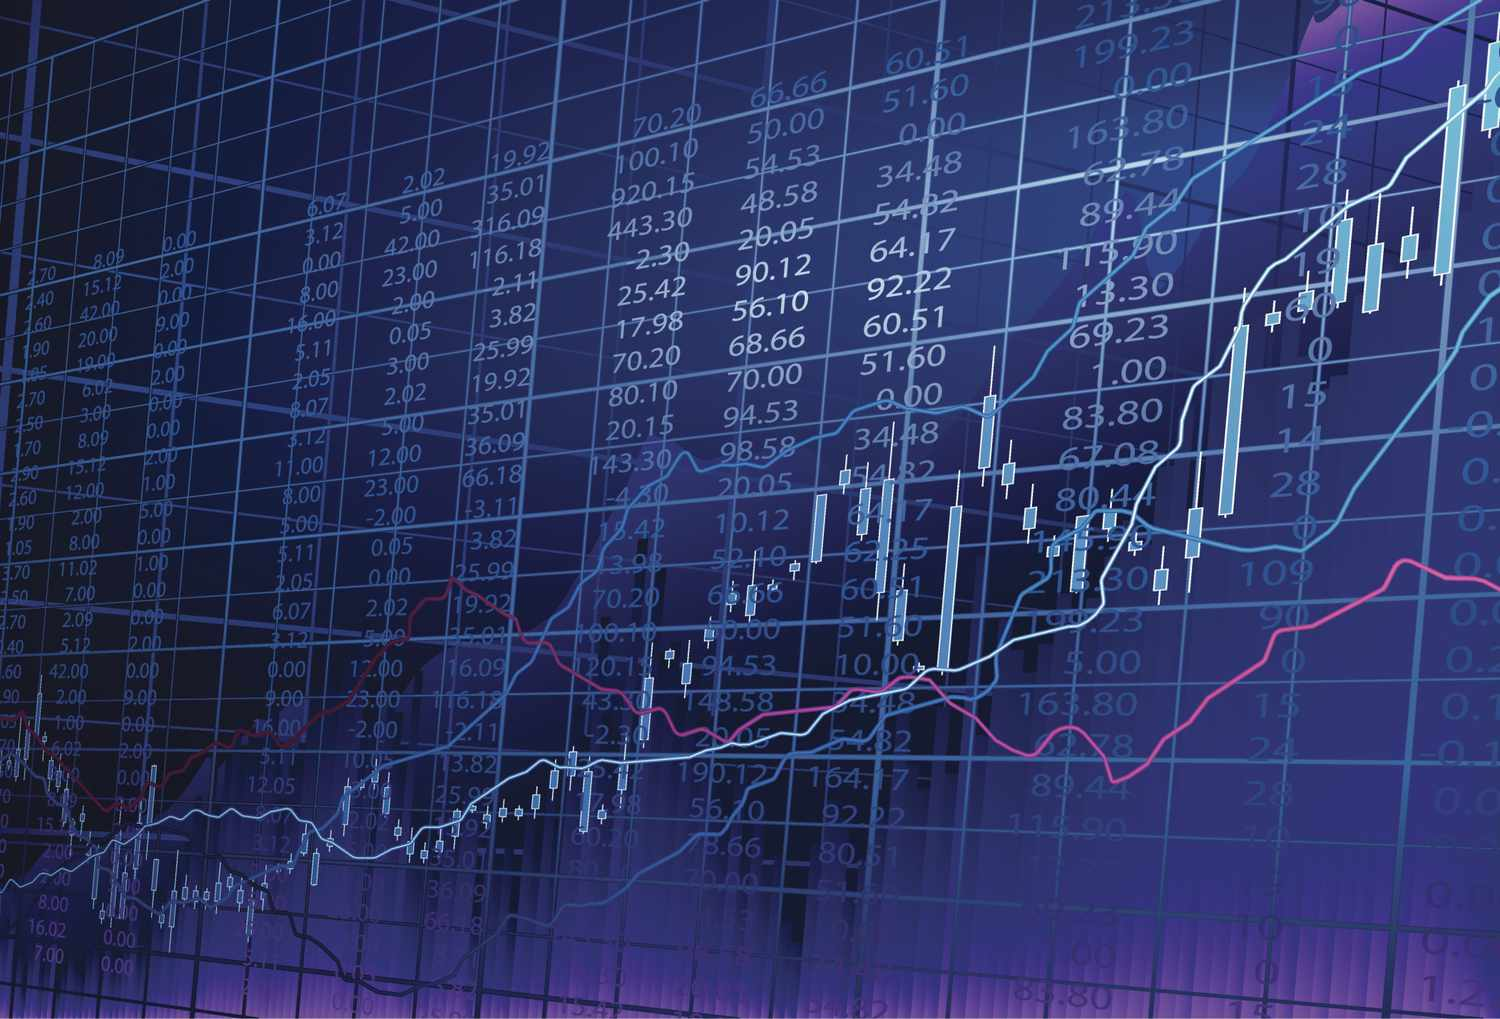
\includegraphics[width=\textwidth]{stock3}
\end{center}


\begin{LARGE}

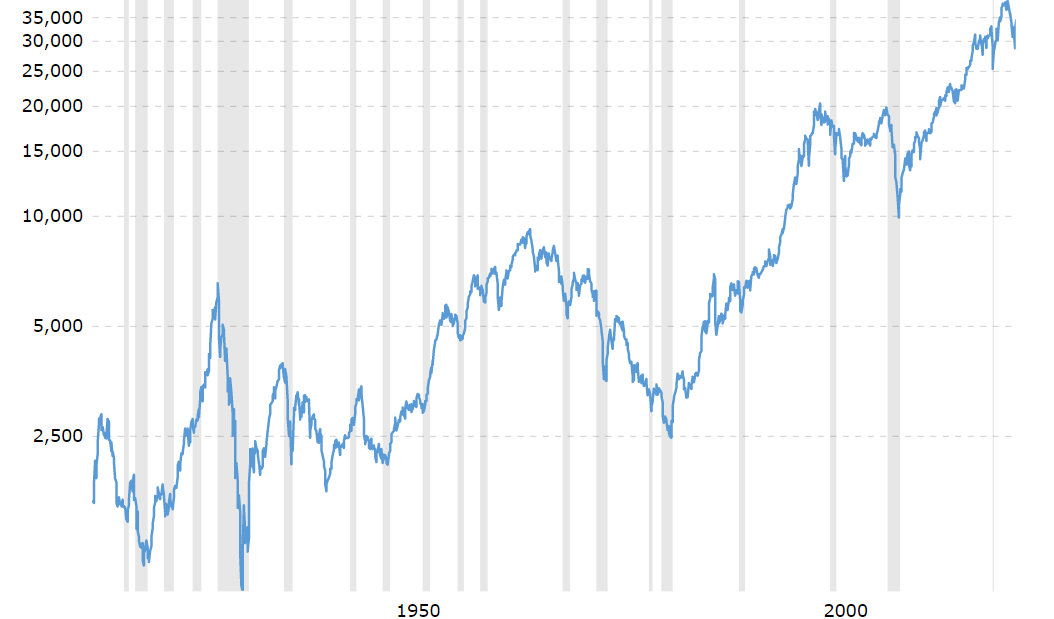
\includegraphics[width=\textwidth]{trends}
\\
Let's look at a table giving description of the BSE TOP GAINERS:
\\
\begin{center}
\begin{tabular}{ ||c c c c|| }
\hline
 securityId & scripCode & LTP \\ 
 \hline
 CHEMPLASTS & 543,336 & 304.60 \\ 
 NETWORK18 & 532,798 & 73.40 \\  
 LTTS & 540,115 & 4,156.15  \\  
 NETWORK18 & 532,798 & 73.40 \\  
 LTTS & 540,115 & 4,156.15    
\end{tabular}
\end{center}
\end{LARGE}
\newpage
\begin{Large}
\begin{center}
NOW, LETS LOOK AT SOME DATA FROM ATHLETES

\csvautotabular{data.csv}

\end{center}


\end{Large}
\end{document}